\documentclass{beamer}
\usepackage[utf8]{inputenc}
\usepackage{listings}
\usepackage{graphicx}
\usetheme{Madrid}
\usecolortheme{beaver}

\input{revision}

\title{Elixir Pipelines}
\subtitle{gen\_stage}
\author[joaohf]{João Henrique Ferreira de Freitas \\ \texttt{https://github.com/joaohf} \\ \texttt{joaof@gmail.com}}
\date[EMC Oct 2018]{Elixir Meetup, Campinas Oct 2018}

\logo{\Revision}

\lstdefinelanguage{elixir}{
	morekeywords={case,catch,def,do,else,false,%
		use,alias,receive,timeout,defmacro,defp,%
		for,if,import,defmodule,defprotocol,%
		nil,defmacrop,defoverridable,defimpl,%
		super,fn,raise,true,try,end,with,%
		unless},
	otherkeywords={<-,->},
	sensitive=true,
	morecomment=[l]{\#},
	morecomment=[n]{/*}{*/},
	morestring=[b]",
	morestring=[b]',
	morestring=[b]"""
}

%\AtBeginSection[]
%{
%  \begin{frame}
%    \frametitle{Table of Contents}
%    \tableofcontents[currentsection]
%  \end{frame}
%}

\begin{document}
  \begin{frame}
    \titlepage
  \end{frame}

  \section[Section]{EIP}

  \begin{frame}
    \frametitle{EIP: Pipes and Filters}

     \begin{figure}[t]
     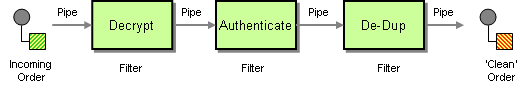
\includegraphics[scale=0.5]{img/PipesAndFilters.png}
     \centering
     \end{figure}
     
     \href{https://www.enterpriseintegrationpatterns.com/patterns/messaging/PipesAndFilters.html}{Message patterns: Pipes and Filters}

  \end{frame}
    
  \begin{frame}
    \frametitle{EIP: Pipes and Filters}
    \framesubtitle{Filters}
    
    Each filter exposes a very simple interface: \pause
    
    \begin{itemize}[<+->]
      \item it receives messages on the inbound pipe,
      \item processes the message,
      \item and publishes the results to the outbound pipe.    
    \end{itemize}
    

  \end{frame}
  
  \begin{frame}
    \frametitle{EIP: Pipes and Filters}
    \framesubtitle{Pipes}

    The pipe connects one filter to the next, \pause

    \begin{itemize}[<+->]
      \item  sending output messages from one filter to the next.
    \end{itemize}
       
  \end{frame}
  
  
  \begin{frame}
    \frametitle{EIP: Pipes and Filters}
    \framesubtitle{Good}

    \begin{itemize}[<+->]
      \item Better runtime properties
      \item Add new processes becomes an easy task
    \end{itemize}
    
  \end{frame}


  \begin{frame}
    \frametitle{EIP: Pipes and Filters}
    \framesubtitle{Odd}
    
    \begin{itemize}[<+->]
      \item  Produces event faster than consumes
      \item  Consumes does not handle event on the right time
      \item  Back pressure (?)
      \item  Concurrency control
    \end{itemize}
  
  \end{frame}
  
  \section[Section]{gen_stage}
  
  \begin{frame}
    \frametitle{GenStage}
    \framesubtitle{as building block}
        
    \begin{block}{}
    Producer and consumer pipelines with back-pressure for Elixir \pause
    \end{block}
    
    \begin{alertblock}{}
    Allow creating processing stages to send and receive data from other stages
    \end{alertblock}
            
  \end{frame}
  
  \begin{frame}
    \frametitle{GenStage}
    \framesubtitle{Back pressure}
    
    \begin{block}{}
    To start the flow of events:
    \begin{itemize}[<+->]
      \item we subscribe consumers to producers,
      \item consumers will ask the producers for events (sending demand upstream),
      \item once demand arrives, the producer will emit items (never emitting more items than the consumer asked for)
    \end{itemize}
     
    \end{block}

    \pause
    
    \begin{alertblock}{} 
    This provides a back-pressure mechanism.
    \end{alertblock} 

  \end{frame}

  \begin{frame}
    \frametitle{GenStage}
    \framesubtitle{Produces and consumers}
        
    \begin{itemize}[<+->]
      \item  Producer: when the stage sends data
      \item  Consumer: when the stage receives data
      \item  Producer-Consumer: send and receive data
    \end{itemize}
    
    \pause
    
    A consumer may have multiple producer and a producer may have multiple consumers.
        
  \end{frame}
  
  \begin{frame}
    \frametitle{GenStages}
    \framesubtitle{Buffering events}
    
    \begin{itemize}[<+->]
      \item the producer will automatically buffer the events
      \item when an event cannot be sent immediately by a producer,
      \item the event will be automatically stored and sent the next time consumers ask for events.
    \end{itemize}
    
    
  \end{frame}


  \begin{frame}
    \frametitle{GenStages}
    \framesubtitle{Buffering demand}
    
    \begin{itemize}[<+->]
      \item In case consumers send demand and the producer is not yet ready to fill in the demand,
      \item producers must buffer the demand until data arrives.
    \end{itemize}

  \end{frame}


  \begin{frame}
    \frametitle{GenStages}
    \framesubtitle{resumo}
    
    \begin{block}{It's all about demand}
    Producing events is just about handling the demand required by consumers
    \end{block}

  \end{frame}
  
  \section[Section]{Real world example}
      
  \begin{frame}
    \frametitle{Real world example}
    \framesubtitle{Eugenio Jaiminho}
    
     \begin{figure}[t]
     
\includegraphics[scale=0.5]{img/jaiminho.png}
     \centering
     \end{figure}
     
  \end{frame}


  \begin{frame}
    \frametitle{Real world example}
    \framesubtitle{Eugenio Jaiminho, functional}
  
  Data Ingestion using:
  \begin{itemize}
    \item http
    \item websocket
  \end{itemize}
  
  Convert external events to Eugenio internal event stream
  \begin{itemize}
    \item JSON
  \end{itemize}
  
  Publish to message broker topics
  \begin{itemize}
    \item Kafka
  \end{itemize}
  
  
  
  \end{frame}
  
  
  \begin{frame}
    \frametitle{Real world example}
    \framesubtitle{Eugenio Jaiminho, non-functional}
     
    \begin{itemize}
      \item metrics
      \item logs
      \item Azure Event Hub with Kafka
      \item Open source Kafka
    \end{itemize}
   
    Runtime:
    \begin{itemize}
      \item Docker container
      \item UCR (Mesos)
    \end{itemize}
   
  \end{frame}
  
  
  \begin{frame}
    \frametitle{Real world example}
    \framesubtitle{Eugenio Jaiminho: elixir}
    
    Regular elixir application:
    \begin{itemize}
      \item mix tool
      \item distillery, to handle release
      \item dev, test, prod
      \item phoenix
      \item gen\_stage
      \item statix
      \item brod
    \end{itemize}

  \end{frame}
  
  
  \begin{frame}
    \frametitle{Eugenio Jaiminho}
    \framesubtitle{Overall design}

     \begin{figure}[t]
     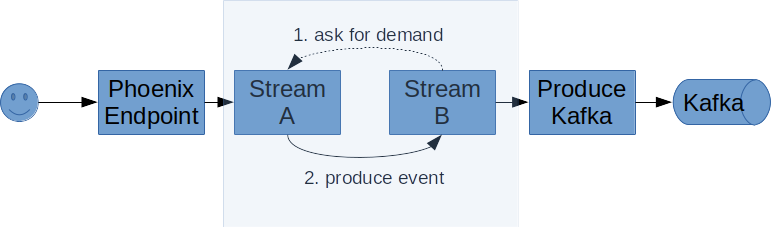
\includegraphics[scale=0.5]{img/design.png}
     \centering
     \end{figure}
     
  \end{frame}


  \begin{frame}
    \frametitle{Eugenio Jaiminho}
    \framesubtitle{Let's test}

     \begin{figure}[t]
     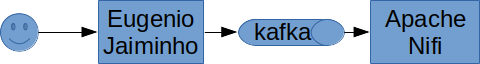
\includegraphics[scale=0.5]{img/test1.png}
     \centering
     \end{figure}
     
     \begin{itemize}
       \item Send event to Eugenio Jaiminho
       \item See at Kafka consumer
     \end{itemize}
     
  \end{frame}

  \begin{frame}
    \frametitle{Flow}
    \framesubtitle{}

    \begin{block}{}
    Flow allows developers to express computations on collections, similar to the Enum and Stream modules, although computations will be executed in parallel using multiple GenStages. https://github.com/plataformatec/flow
    \end{block}
    
  \end{frame}

  \begin{frame}
    \frametitle{References}
    \framesubtitle{}
    
    \begin{itemize}
    \item \href{https://github.com/elixir-lang/gen_stage}{gen\_stage: Producer and consumer pipelines with back-pressure for Elixir}
    \item \href{https://www.youtube.com/watch?v=6gcsjCl9ne0}{ElixirConf 2018 - Using Elixir GenStage to Track Video Watch Progress - Emerson Macedo}
    \item \href{https://www.youtube.com/watch?v=trpueWn8DIM}{Realtime Data Pipelines with Elixir GenStage - Peter Hasti}
    \item \href{https://www.youtube.com/watch?v=XPlXNUXmcgE}{GenStage and Flow - José Valim (Lambda Days 2017)}
    \item \href{https://blog.emerleite.com/using-elixir-genstage-to-track-video-watch-progress-9b114786c604}{Using Elixir GenStage to track Video Watch Progress}
    \item \href{https://github.com/plataformatec/flow}{Flow: Computational parallel flows on top of GenStage}
    \end{itemize}

  \end{frame}


    \begin{frame}
    \begin{center}
    \Huge Thank You!
    \end{center}
  \end{frame}
    
  \begin{frame}
    \frametitle{Colophon}    
    \begin{itemize}
    \item Latex
    \item Beamer
    \item Texmaker
    \end{itemize}    
  \end{frame}


\end{document}
